\documentclass[25pt, a0paper, portrait, blockverticalspace=1.5cm]{tikzposter}
\usetikzlibrary{positioning}

\title{\parbox{\linewidth}{\centering SPIN DECOHERENCE IN THE FROZEN SPIN STORAGE RING METHOD OF SEARCH FOR A PARTICLE EDM}}
\author{A.E. Aksentyev\textsuperscript{1,2,3}, Y.V. Senichev\textsuperscript{3}}
\institute{
  \textsuperscript{1} National Research Nuclear University ``MEPhI,'' Moscow, Russia \\
  \textsuperscript{2} Institut f\"ur Kernphysik, Forschungszentrum J\"ulich, J\"ulich, Germany\\
  \textsuperscript{3} Institute for Nuclear Research of the Russian Academy of Sciences, Moscow, Russia
}


\usetheme{Simple}
\usecolorstyle{Russia}
\colorlet{blocktitlefgcolor}{black}

\usepackage{mathtools}
\usepackage{amsmath}
\usepackage{xparse}
\usepackage{caption}
\captionsetup{font=large}
\usepackage{multicol}
\setlength\columnsep{1.5cm}


\let\oldvec\vec
\renewcommand{\vec}{\boldsymbol}
\DeclareDocumentCommand{\bkt}{sm}{\IfBooleanTF{#1}{\left[ #2 \right]}{\left(#2\right)}}
\DeclareDocumentCommand{\ddt}{m}{\frac{\mathrm{d} {#1}}{\mathrm{d} t}}
\DeclareDocumentCommand{\pddx}{mO{t}O{}}{\frac{\partial^{#3} {#1}}{\partial {#2}^{#3}}}
\newcommand{\w}{\omega}
\newcommand{\W}{\Omega}
\newcommand{\subwidth}{.9\linewidth}
\newcommand{\D}{\Delta}
\newcommand{\const}{\mathrm{const}}
\newcommand{\nbar}{\bar n}

\begin{document}

\maketitle

\block{INTRODUCTION}{
  \begin{multicols}{3}
    Spin coherence refers to a measure of preservation of polarization in an initially polarized beam.
    The spin vector of a particle injected into a storage ring starts to precess about
    the vertical magnetic field vector in accordance with the Thomas-BMT equation.\columnbreak

    The precession frequency
    is dependent on the equilibrium-level energy, which differs across the beam particles.
    This does not pose a problem when the initial polarization is vertical; however,
    the Frozen Spin Storage Ring EDM search method requires beam polarization along the momentum vector,
    i.e., in the horizontal plane. \columnbreak
    
    In the present work we analyze the source of decoherence, and investigate the way it can be suppressed
    in the horizontal plane in a perfectly aligned ring by means of sextupole fields. We also consider
    the case of an imperfect ring: transference of decoherence into the vertical plane induced by vertical
    plane spin precession, and the effect of sextupole fields.
  \end{multicols}
}

\begin{columns}
  \column{.5}
  \block[bodyoffsety=2cm, titleoffsety=2cm]{ORIGIN OF DECOHERENCE}{
    A particle's spin tune depends on its equilibrium-level energy, expressed by the Lorentz factor:
    \begin{equation*}\label{eq:spin_tune_vs_gamma}
      \begin{cases}
        \nu_s^B &= \gamma G, \\
        \nu_s^E &= \frac{G+1}{\gamma} - \gamma G.
      \end{cases}
    \end{equation*}
    
    As a consequence of the phase stability principle, particles having longer orbits must
    possess higer equilibrium energy levels; else they'd fall from the bunch.

    \begin{minipage}[b]{.5\linewidth}
      \begin{tikzfigure}
        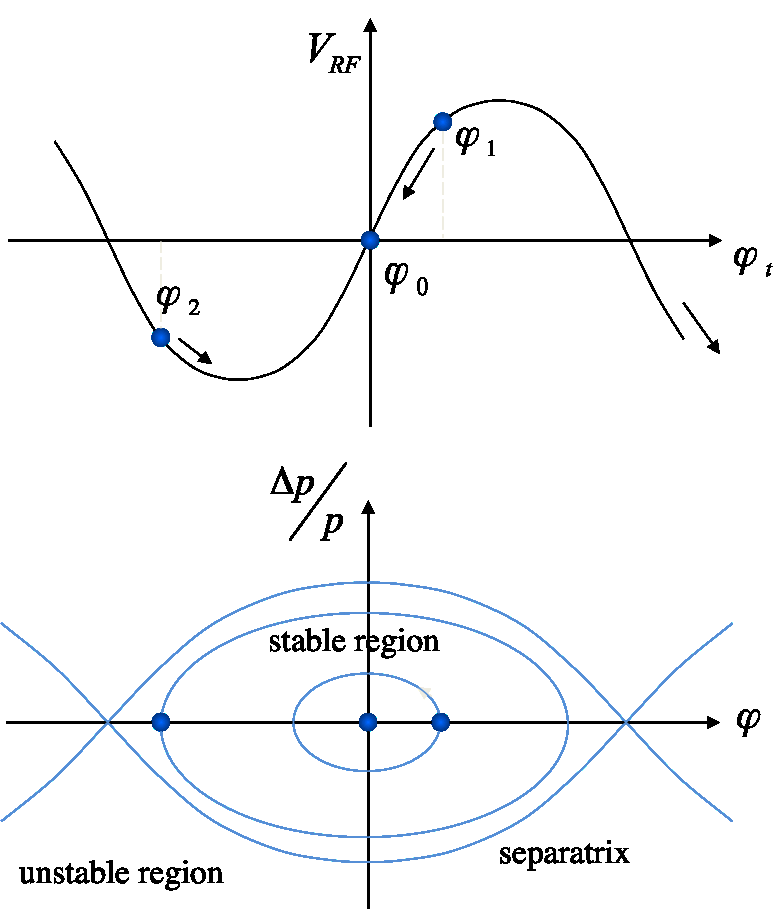
\includegraphics[width=\linewidth]{../img/SEMINAR/psp_diagram}
      \end{tikzfigure}
      \captionof{figure}{Linear theory}
    \end{minipage}
    \begin{minipage}[b]{.5\linewidth}
      \begin{tikzfigure}
        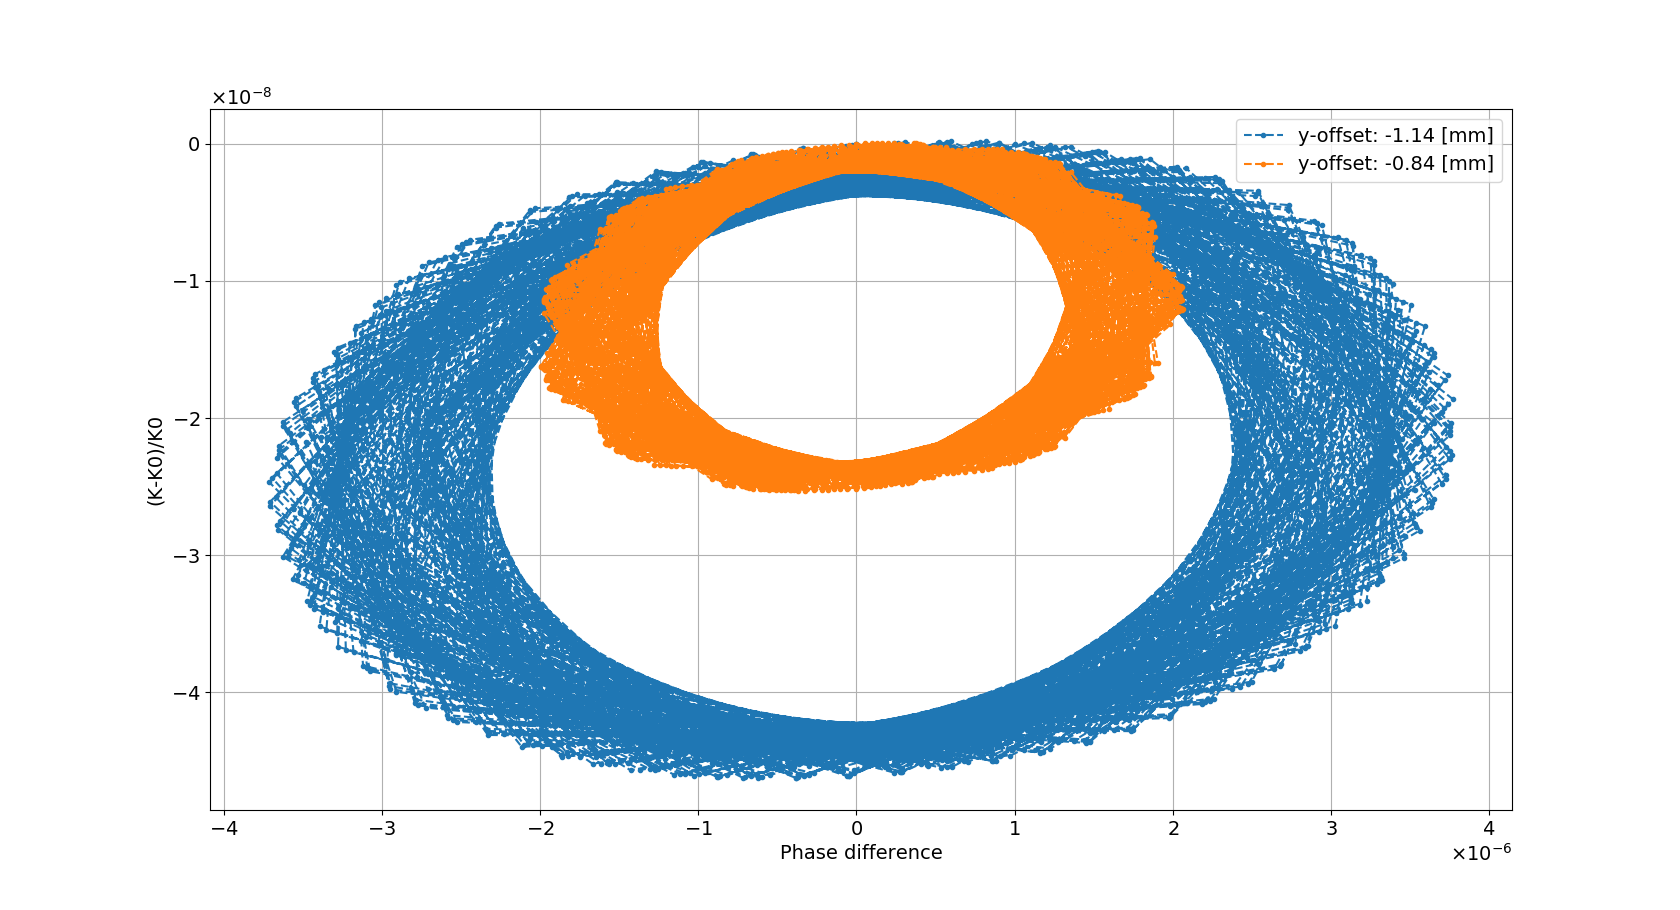
\includegraphics[width=\linewidth]{../img/SEMINAR/psp_diagram_betatron}
      \end{tikzfigure}
      \captionof{figure}{3rd order transfer maps. Observe equilibrium level energy offset}
    \end{minipage}
  }
  \block{PERFECT LATTICE}{
    \begin{minipage}{.5\linewidth}
      \begin{itemize}
      \item Beam energy 270 MeV;
      \item spin precession axis $\nbar = \hat y$;
      \item $\nu_s(z) = \sum_{k=0}^5 a_k\cdot z^k + O(z^6)$;
      \item minimize coefficient $a_2$ to remove quadratic dependence.
      \end{itemize}
    \end{minipage}
    \begin{minipage}{.5\linewidth}
      \begin{tikzfigure}
        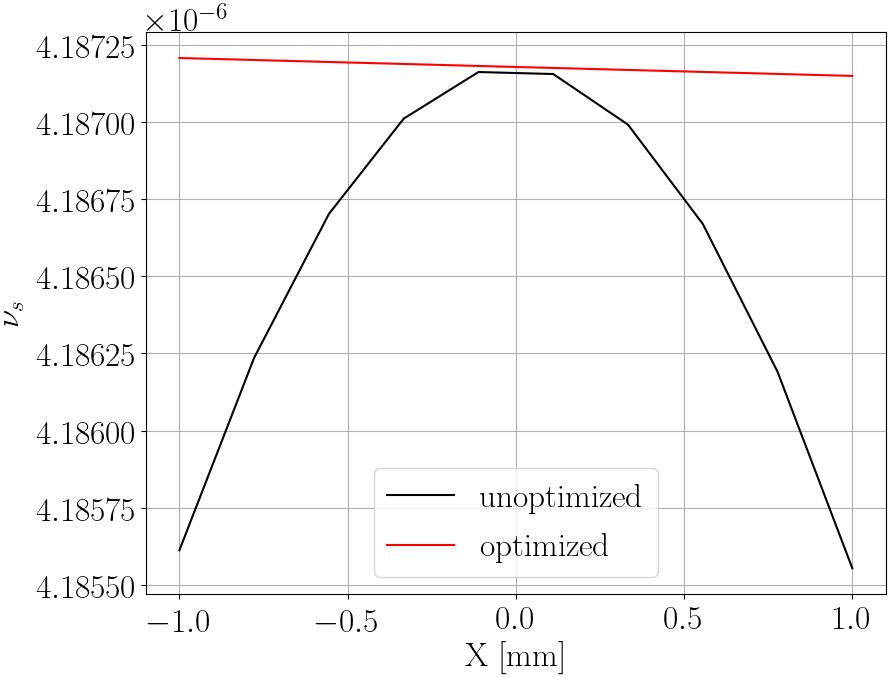
\includegraphics[width=\linewidth]{../img/IPAC19/spin_tune_decoh_x_offset}
      \end{tikzfigure}
      \captionof{figure}{Spin tune dependence on horizontal offset}
    \end{minipage}
    \begin{minipage}{.5\linewidth}
      \begin{tikzfigure}
        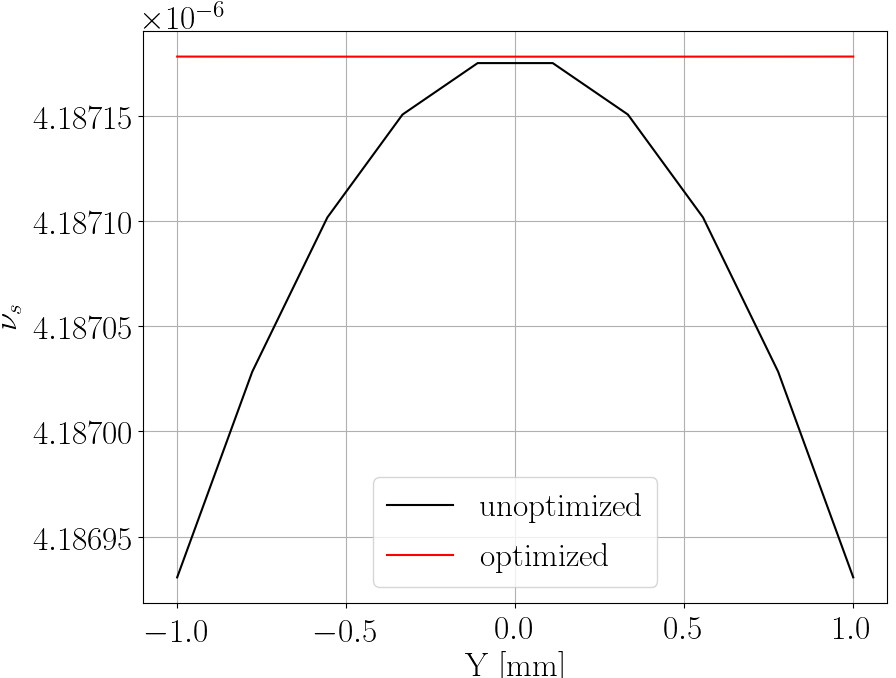
\includegraphics[width=\linewidth]{../img/IPAC19/spin_tune_decoh_y_offset}
      \end{tikzfigure}
      \captionof{figure}{Spin tune dependence on vertical offset}
    \end{minipage}~~~~~~
    \begin{minipage}{.5\linewidth}
      \begin{tikzfigure}
        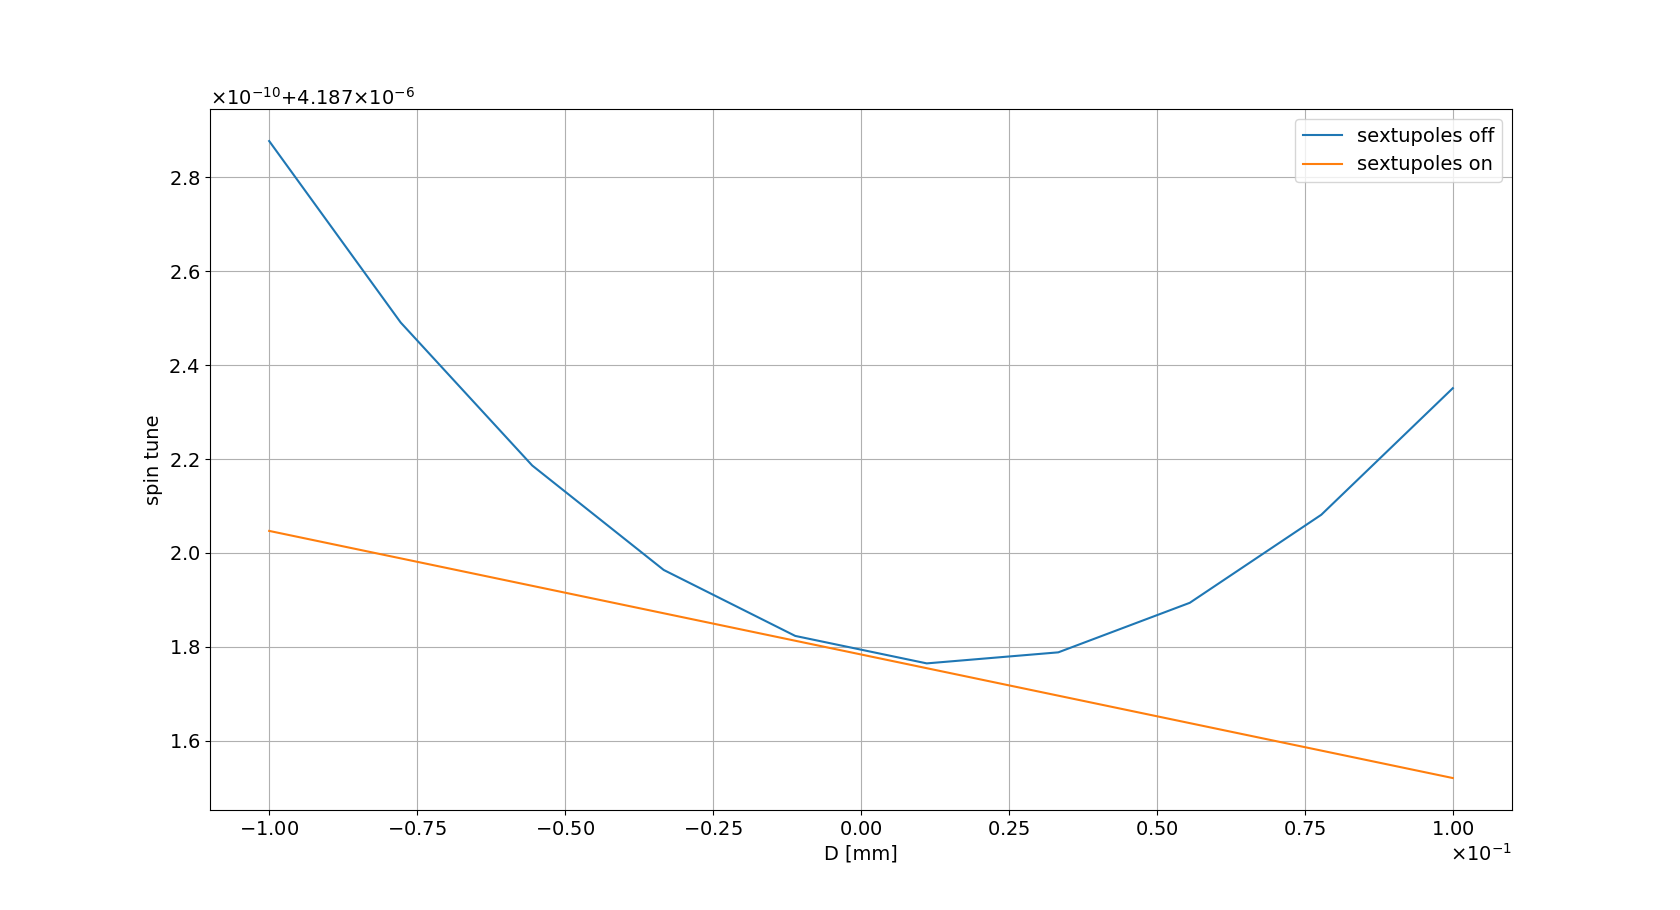
\includegraphics[width=\linewidth]{../img/IPAC19/spin_tune_decoh_d_offset}
      \end{tikzfigure}
      \captionof{figure}{Spin tune dependence on energy offset}
    \end{minipage}
  }
  
  \column{.5}
  \block[bodyoffsety=2cm, titleoffsety=2cm]{EFFEFCTIVE LORENTZ FACTOR}{
    Betatron motion orbit lengthening and synchrotron oscillations cause an equilibrium-level momentum shift
    \begin{equation*}\label{eq:EquLevMom_shift}
      \Delta\delta_{eq} = \frac{\gamma_0^2}{\gamma_0^2\alpha_0 - 1}\bkt*{\frac{\delta_m^2}{2}\bkt{\alpha_1 - \alpha_0\gamma^{-2} + \gamma_0^{-4}} + \bkt{\frac{\Delta L}{L}}_\beta},
    \end{equation*}
    where $\delta_m$ is the amplitude of synchrotron oscillations.\\
    
    The corresponding \emph{effective} Lorentz factor
    \begin{equation*}\label{eq:EffectiveGamma}
      \gamma_{eff} = \gamma_0 + \beta_0^2\gamma_0\cdot\Delta\delta_{eq},
    \end{equation*}
    where $\gamma_0$, $\beta_0$ are the Lorentz factor and normalized speed of the reference particle.
  }
  \block{SEXTUPOLE DECOHERENCE SUPPRESSION}{
      %% \begin{tabular}{lr}
      %%   A sextupole of strength & $S_{sext} = \frac{1}{B\rho} \pddx{B_y}[x][2]$\\ & \\
      %%   modifies both the momentum compaction factor & $\Delta \alpha_{1,sext} = -\frac{S_{sext}D_0^3}{L}$\\ & \\
      %%   and the particle orbit length & $\bkt{\frac{\Delta L}{L}}_{sext} = \mp \frac{S_{sext}D_0\beta_{x,y}\varepsilon_{x,y}}{L}$\\
      %% \end{tabular}

    A sextupole of strength
    \begin{align*}
      S_{sext} &= \frac{1}{B\rho} \pddx{B_y}[x][2]
      \intertext{modifies both the momentum compaction factor}
      \Delta \alpha_{1,sext} &= -\frac{S_{sext}D_0^3}{L},
      \intertext{and the particle orbit length}
      \bkt{\frac{\Delta L}{L}}_{sext} &= \mp \frac{S_{sext}D_0\beta_{x,y}\varepsilon_{x,y}}{L}.
    \end{align*}
    \newline
    Here
    $
    D(s,\delta) = D_0(s) + D_1(s)\delta
    $
    is the dispersion function.
  }
  \block[bodyoffsety=1.5cm, titleoffsety=1.5cm]{IMPERFECT LATTICE}{
    \begin{minipage}{.5\linewidth}
      \begin{tikzfigure}
        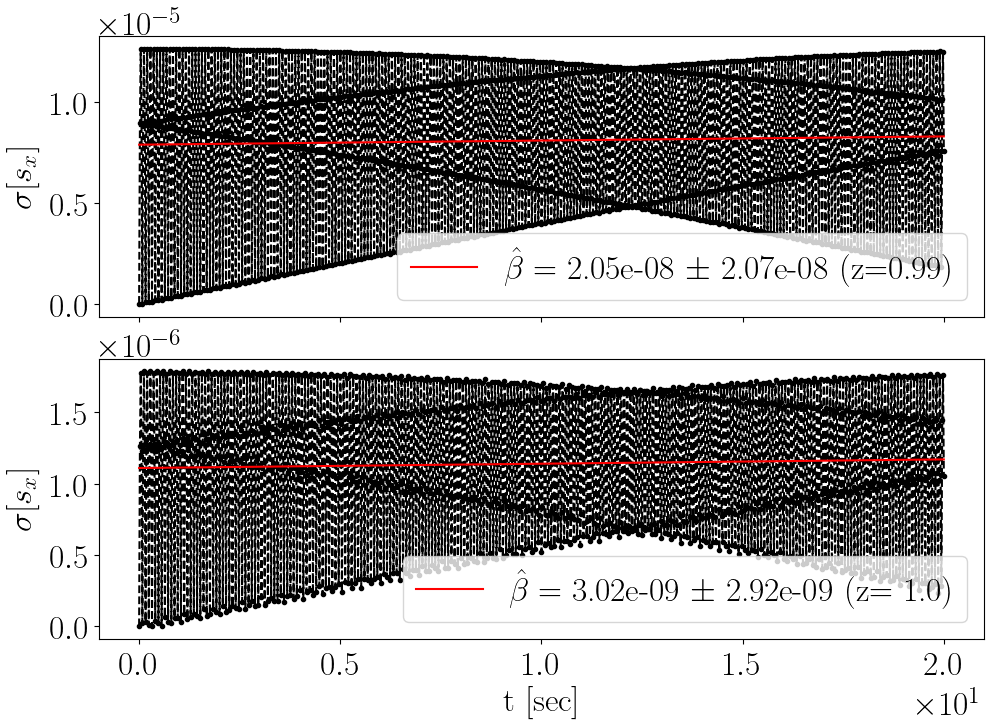
\includegraphics[width=\linewidth]{../img/IPAC19/SX_decoh_20sec_both}
      \end{tikzfigure}
      \captionof{figure}{Decoherence in the horizontal plane.
        Top panel: sextupoles are off; bottom panel: sextupoles are on.}
    \end{minipage}~~~~~~
    \begin{minipage}{.5\linewidth}
      \begin{tikzfigure}
        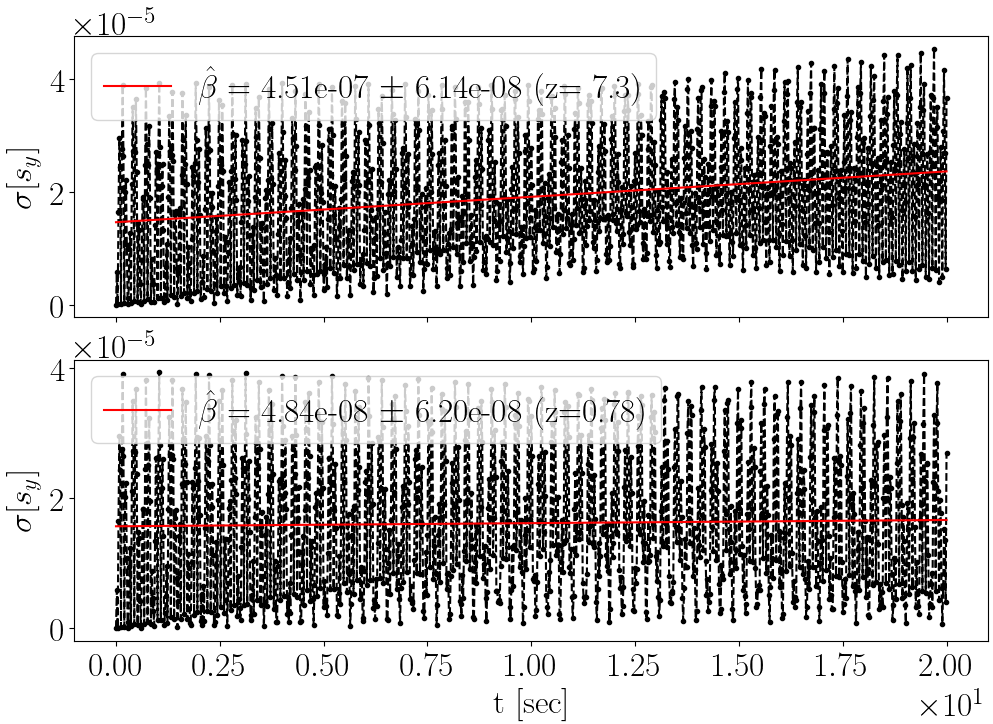
\includegraphics[width=\linewidth]{../img/IPAC19/SY_decoh_20sec_both}
      \end{tikzfigure}
      \captionof{figure}{Decoherence in the vertical plane.
        Top panel: sextupoles are off; bottom panel: sextupoles are on.}
    \end{minipage}
  }
  \block{CONCLUSIONS}{
    \begin{enumerate}
    \item Orbit lengthening and momentum deviation cause spin decoherence via equilibrium level momentum shift;
    \item In an imperfect lattice, there's no decoherence in the horizontal plane,
      but it transfers into the vertical plane;
    \item Sextupole fields suppress decoherence by removing the parabolic dependence of spin tune on particle
      phase space coordinates;
    \item Linear decoherence effects need further study; the working hypothesis is that they can be
      suppressed by adjusting the RF cavity parameters.
    \end{enumerate}
  }

  %% \block{REFERENCES}{
  %%   \begin{thebibliography}{9}
  %%   \bibitem{Eremey:Thesis}
  %%     E. Valetov, ``Field modeling, symplectic tracking, and spin decoherence for the EDM and muon g-2 lattices,''
  %%     PhD thesis, Dept. of Phys. and Astr., Michigan State University, East Lansing, Michigan, USA.
  %%     %% \url{http://collaborations.fz-juelich.de/ikp/jedi/public_files/theses/valetovphd.pdf}
  %%   \end{thebibliography}
  }
\end{columns}


\end{document}
